\documentclass[12pt]{article}

% Use packages %
\usepackage{graphicx, courier, amsmath, amssymb, amscd, amsfonts, mathtools, bm, esint, leftidx, extarrows, latexsym, relsize, color, tikz, comment, stmaryrd, float}
\usepackage[obeyspaces]{url}% http://ctan.org/pkg/url

% Set length %
\setlength{\textwidth}{160mm}
\setlength{\textheight}{235mm}
\setlength{\oddsidemargin}{-0mm}
\setlength{\topmargin}{-10mm}

% Define h-bar %
\newsavebox{\myhbar}
\savebox{\myhbar}{$\hbar$}
\renewcommand*{\hbar}{\mathalpha{\usebox{\myhbar}}}

% Chinese input %
%\usepackage{xeCJK} 
%\setCJKmainfont{微軟正黑體}
%\usepackage[T1]{fontenc}
%\makeatletter

% Equation number %
%\@addtoreset{equation}{section} 
%\renewcommand\theequation{{\thesection}.{\arabic{equation}}}
%\makeatletter 

% Helper Command %
\newcommand{\argmin}{\operatornamewithlimits{argmin}}
\newcommand{\rmnum}[1]{\romannumeral #1} 
\newcommand{\Rmnum}[1]{\expandafter\@slowromancap\romannumeral #1@}
\newcommand{\overbar}[1]{\mkern 1.5mu\overline{\mkern-1.5mu#1\mkern-1.5mu}\mkern 1.5mu}
\makeatother
\newcommand*{\QEDA}{\hfill\ensuremath{\blacksquare}}
\newcommand*{\QEDB}{\hfill\ensuremath{\square}}
\newcommand*{\BmVert}{\bigm\vert}
\newcommand{\bigslant}[2]{{\raisebox{.2em}{$#1$}\left/\raisebox{-.2em}{$#2$}\right.}}
\newcommand{\Nelements}[3]{\left\{ #1, ~ #2, \ldots, ~ #3 \right\}}
\newcommand{\CBrackets}[1]{\left\{#1\right\}}
\newcommand{\SBrackets}[1]{\left[#1\right]}
\newcommand{\BooBrackets}[1]{\left\llbracket#1\right\rrbracket}
\newcommand{\ParTh}[1]{\left(#1\right)}
\newcommand{\Ceil}[1]{\left\lceil#1\right\rceil}
\newcommand{\Floor}[1]{\left\lfloor#1\right\rfloor}
\newcommand{\BF}[1]{{\bf#1}}
\newcommand{\Inverse}[1]{{#1}^{-1}}
\newcommand{\Generator}[1]{\left\langle#1\right\rangle}
\newcommand{\AbsVal}[1]{\left|#1\right|}
\newcommand{\VecAbsVal}[1]{\left\|#1\right\|}
\newcommand{\BSlash}[2]{\left.#1\middle\backslash#2\right.}
\newcommand{\Divide}[2]{\left.#1\middle/#2\right.}
\newcommand{\SciNum}[2]{#1\times{10}^{#2}}
\newcommand{\Matrix}[2]{\SBrackets{\begin{array}{#1}#2\end{array}}}
\newcommand{\MatrixTwo}[4]{\ParTh{\begin{array}{cc}{#1}&{#2}\\{#3}&{#4}\end{array}}}
\newcommand{\MatrixNByN}[1]{\Matrix{cccc}{{#1}_{11} & {#1}_{12} & \cdots & {#1}_{1n} \\ {#1}_{21} & {#1}_{22} & \cdots & {#1}_{2n} \\ \vdots & \vdots & \ddots & \vdots \\ {#1}_{n1} & {#1}_{n2} & \cdots & {#1}_{nn}}}
\newcommand{\ndiv}{\hspace{-4pt}\not|\hspace{2pt}}
\newcommand{\eqdef}{\xlongequal{\text{def}}}%
\newcount\arrowcount
\newcommand\arrows[1]{\global\arrowcount#1 \ifnum\arrowcount>0
\begin{matrix}\expandafter\nextarrow\fi}
\newcommand\nextarrow[1]{\global\advance\arrowcount-1 \ifx\relax#1\relax\else \xrightarrow{#1}\fi\ifnum\arrowcount=0 \end{matrix}\else\\\expandafter\nextarrow\fi}
\newcommand{\horrule}[1]{\rule{\linewidth}{#1}}

% Tikz settings %
\usetikzlibrary{shapes,arrows}
\tikzstyle{decision} = [diamond, draw, fill=white!20, text width=4.5em, text badly centered, node distance=3cm, inner sep=0pt]
\tikzstyle{block}    = [rectangle, draw, fill=white!20, text width=8em, text centered, rounded corners, minimum height=4em]
\tikzstyle{point}    = [fill = white!20, minimum size=0.5cm]
\tikzstyle{line}     = [draw, -latex']
\tikzstyle{mapsto}   = [draw, |->]
\tikzstyle{cloud}    = [draw, ellipse,fill=red!20, node distance=3cm, minimum height=2em]

\begin{document}

\baselineskip 6.5mm
\setlength{\parindent}{0pt}
\title{ 
\normalfont \normalsize 
\horrule{0.5pt} \\[0.4cm]
\huge { \Huge Machine Learning \\ \large Answer Sheet for Homework 5 }\\ % The assignment title
\horrule{2pt} \\ [0.5cm]
}
\author{ { \Large Da-Min HUANG } \\
{\small R04942045} \\
{\small\textit{Graduate Institute of Communication Engineering, National Taiwan University}}
}
\date{December 9, 2015}
%\allowdisplaybreaks[4]
\maketitle

\subsection*{Problem 1}

The hard-margin support vector machine is with $d+1$ variables. For soft-margin support vector machine, there are $N$ more variables $\xi_n$, $1\leq n\leq N$.

So soft-margin support vector machine is a quadratic programming problem with $N+d+1$ variables.

\QEDB

\horrule{0.5pt}

\subsection*{Problem 2}

I wrote a \url{Q02.py} to help me get the answer. By using Python package \url{cvxopt}$^{[2]}$, with
\begin{align}
\BF{z}=\Matrix{rr}{1&-2\\4&-5\\4&-1\\5&-2\\7&-7\\7&1\\7&1}, \BF{y}=\Matrix{c}{-1\\-1\\-1\\+1\\+1\\+1\\+1}
\end{align}
and
\begin{align}
\BF{Q}&=\Matrix{ccc}{0&0&0\\0&1&0\\0&0&1},\BF{p}=\Matrix{c}{0\\0\\0},\\
\BF{A}^T&=\Matrix{rrr}{-1&-1&2\\-1&-4&5\\-1&-4&1\\1&5&-2\\1&7&-7\\1&7&1\\1&7&1},\BF{c}=\Matrix{c}{1\\1\\1\\1\\1\\1\\1}
\end{align}
To use this package, I gave \url{solvers.qp(}$\BF{Q}, \BF{p}, -\BF{A}^T, -\BF{c}$\url{)} and got
\begin{align}
b=-9,\BF{w}=\SBrackets{2,0}
\end{align}
So the hyperplane is
\begin{align}
2z_1-9=0\Rightarrow z_1=4.5
\end{align}

\QEDB

\horrule{0.5pt}

\subsection*{Problem 3}

I wrote a \url{Q03.py} to help me get the answer. By using Python package \url{cvxopt}, with
\begin{align}
\BF{Q}&=\Matrix{rrrrrrr}{4&1&1&0&-1&-1&-1\\1&4&0&-1&-9&-1&-1\\1&0&4&-1&-1&-9&-1\\0&-1&-1&4&1&1&9\\-1&-9&-1&1&25&9&1\\-1&-1&-9&1&9&25&1\\-1&-1&-1&9&1&1&25},\BF{p}=\Matrix{r}{-1\\-1\\-1\\-1\\-1\\-1\\-1},\\
-\BF{A}^T&=\Matrix{rrrrrrr}{-1&0&0&0&0&0&0\\0&-1&0&0&0&0&0\\0&0&-1&0&0&0&0\\0&0&0&-1&0&0&0\\0&0&0&0&-1&0&0\\0&0&0&0&0&-1&0\\0&0&0&0&0&0&-1},\BF{c}=\Matrix{c}{0\\0\\0\\0\\0\\0\\0}
\end{align}
with
\begin{align}
\BF{G}=\BF{y}^T=\Matrix{ccccccc}{-1&-1&-1&1&1&1&1}\text{ and }h=0
\end{align}
and
To use this package, I gave \url{solvers.qp(}$\BF{Q}, \BF{p}, -\BF{A}^T, \BF{c},\BF{G},h$\url{)} and got
\begin{align}
\alpha=\SBrackets{\SciNum{4.32}{-9}\approx0,0.704,0.704,0.889,0.259,0.259,\SciNum{5.27}{-10}\approx0}
\end{align}
where \url{cvxopt} needs conditions
\begin{align}
-\BF{A}^T{\bm\alpha}\preceq\BF{c}\text{ and }\BF{G}\bm{\alpha}=h
\end{align}

Support vectors are the corresponding $\alpha_i\neq0$, so $\BF{x}_2$, $\BF{x}_3$, $\BF{x}_4$, $\BF{x}_5$ and $\BF{x}_6$ are support vectors.

\QEDB

\horrule{0.5pt}

\subsection*{Problem 4}

I wrote a \url{Q04.py} to help me get the answer. By using python package \url{sympy} and
\begin{align}
\BF{w}&=\sum_{n=1}^{N}\alpha_ny_nK\ParTh{\BF{x}_n,\Matrix{c}{x_1\\x_2}}+b\\
b&=y_s-\sum_{n=1}^{N}\alpha_ny_nK\ParTh{\BF{x}_n,\BF{x}_s}
\end{align}
we have
\begin{align}
\BF{w}=\dfrac{1}{9}\ParTh{8x^2_1 - 16x_1 + 6x^2_2-15}
\end{align}

\QEDB

\horrule{0.5pt}

\subsection*{Problem 5}

Since kernel function $K\ParTh{\BF{x},\BF{x}^\prime}=\ParTh{1+\BF{x}^T\BF{x}^\prime}^2$ is different from $\BF{z}=\ParTh{\phi\ParTh{\BF{x}},\phi\ParTh{\BF{x}}}$, the curves should be different in the $\mathcal{X}$ space.

\QEDB

\horrule{0.5pt}

\subsection*{Problem 6}

Since $\VecAbsVal{\BF{x}_n-\BF{c}}^2\leq R^2$, $\forall n$, the constraint to maximize is
\begin{align}
\VecAbsVal{\BF{x}_n-\BF{c}}^2-R^2\leq0
\end{align}
so $L\ParTh{R,\BF{c},\bm{\lambda}}$ is
\begin{align}
L\ParTh{R,\BF{c},\bm{\lambda}}=R^2+\sum_{n=1}^{N}\lambda_n\ParTh{\VecAbsVal{\BF{x}_n-\BF{c}}^2-R^2}
\end{align}

\QEDB

\horrule{0.5pt}

\subsection*{Problem 7}

At the optimal $(R,\BF{c},\bm{\lambda})$,
\begin{align}
\dfrac{\partial L}{\partial R}&=2R-2R\sum_{n=1}^{N}\lambda_n=0\Rightarrow\sum_{n=1}^{N}\lambda_n=1\text{ or }R=0\\
\label{KKTC}
\dfrac{\partial L}{\partial\BF{c}}&=2\sum_{n=1}^{N}\lambda_{n}\ParTh{\BF{c}-\BF{x}_{n}}=\BF{0}\Rightarrow\BF{c}=\Divide{\ParTh{\sum_{n=1}^{N}\lambda_n\BF{x}_n}}{\ParTh{\sum_{n=1}^{N}\lambda_n}}\text{ if }\sum_{n=1}^{N}\lambda_n\neq0
%\Rightarrow\lambda_n=0\text{ or }\BF{x}_n=\BF{c}
\end{align}
So the KKT conditions are
\begin{enumerate}
	\item primal feasible: $\VecAbsVal{\BF{x}_n-\BF{c}}^2\leq R^2$.
	\item dual feasible: $\lambda_n\geq0$.
	\item dual-inner optimal: if $R\neq0$, $\sum_{n=1}^{N}\lambda_n=1$ and $\BF{c}=\sum_{n=1}^{N}\lambda_n\BF{x}_n$.
	\item primal-inner optimal: $\lambda_n\ParTh{\VecAbsVal{\BF{x}_n-\BF{c}}^2-R^2}=0$.
\end{enumerate}

\QEDB

\horrule{0.5pt}

\subsection*{Problem 8}

From Problem 6, we have
\begin{align}
L\ParTh{R,\BF{c},\bm{\lambda}}&=R^2+\sum_{n=1}^{N}\lambda_n\ParTh{\VecAbsVal{\BF{x}_n-\BF{c}}^2-R^2}=R^2+\sum_{n=1}^{N}\lambda_n\VecAbsVal{\BF{x}_n-\BF{c}}^2-\sum_{n=1}^{N}\lambda_nR^2\\
&=R^2-R^2+\sum_{n=1}^{N}\lambda_n\VecAbsVal{\BF{x}_n-\BF{c}}^2=\sum_{n=1}^{N}\lambda_n\VecAbsVal{\BF{x}_n-\BF{c}}^2
\end{align}
where $\sum_{n=1}^{N}\lambda_n=1$ since $R\neq0$.

Also, from (\ref{KKTC}), we have $\BF{c}=\sum_{n=1}^{N}\lambda_n\BF{x}_n$. Hence
\begin{align}
\text{Objective}\ParTh{\lambda}=\sum_{n=1}^{N}\lambda_n\VecAbsVal{\BF{x}_n-\sum_{m=1}^{N}\lambda_m\BF{x}_m}^2
\end{align}

\QEDB

\horrule{0.5pt}

\subsection*{Problem 9}

We have
\begin{align}
\sum_{n=1}^{N}\lambda_n\VecAbsVal{\BF{x}_n-\BF{c}}^2&=\sum_{n=1}^{N}\lambda_n\ParTh{\BF{x}^T_n\BF{x}_n-\BF{x}^T_n\BF{c}-\BF{c}^T\BF{x}_n+\BF{c}^T\BF{c}}\\
&=\sum_{n=1}^{N}\lambda_n\ParTh{\BF{x}^T_n\BF{x}_n-\BF{x}^T_n\sum_{m=1}^{N}\lambda_m\BF{x}_m-\ParTh{\sum_{m=1}^{N}\lambda_m\BF{x}_m}^T\BF{x}_n+\VecAbsVal{\sum_{m=1}^{N}\lambda_m\BF{x}_m}^2}
\end{align}
So
\begin{align}
&\sum_{n=1}^{N}\lambda_n\VecAbsVal{\phi\ParTh{\BF{x}_n}-\phi\ParTh{\BF{c}}}^2\\
=&\sum_{n=1}^{N}\lambda_nK\ParTh{\BF{x}_n,\BF{x}_n}-2\sum_{n=1}^{N}\sum_{m=1}^{N}\lambda_n\lambda_mK\ParTh{\BF{x}_n,\BF{x}_m}+\sum_{n=1}^{N}\sum_{m=1}^{N}\lambda_n\lambda_mK\ParTh{\BF{x}_n,\BF{x}_m}\\
=&\sum_{n=1}^{N}\lambda_nK\ParTh{\BF{x}_n,\BF{x}_n}-\sum_{n=1}^{N}\sum_{m=1}^{N}\lambda_n\lambda_mK\ParTh{\BF{x}_n,\BF{x}_m}
\end{align}

\QEDB

\horrule{0.5pt}

\subsection*{Problem 10}

From primal-inner optimal condition, pick some $\lambda_i>0$, we have
\begin{align}
\VecAbsVal{\BF{x}_i-\BF{c}}^2=R^2
\end{align}
so
\begin{align}
R^2&=\BF{x}^T_i\BF{x}_i-\BF{x}^T_i\sum_{m=1}^{N}\lambda_m\BF{x}_m-\ParTh{\sum_{m=1}^{N}\lambda_m\BF{x}_m}^T\BF{x}_i+\sum_{n=1}^{N}\sum_{m=1}^{N}\lambda_n\lambda_m\BF{x}^T_n\BF{x}_m\\
&=K\ParTh{\BF{x}_i,\BF{x}_i}-2\sum_{m=1}^{N}\lambda_mK\ParTh{\BF{x}_i,\BF{x}_m}+\sum_{n=1}^{N}\sum_{m=1}^{N}\lambda_n\lambda_mK\ParTh{\BF{x}_n,\BF{x}_m}\\
\Rightarrow R&=\sqrt{K\ParTh{\BF{x}_i,\BF{x}_i}-2\sum_{m=1}^{N}\lambda_mK\ParTh{\BF{x}_i,\BF{x}_m}+\sum_{n=1}^{N}\sum_{m=1}^{N}\lambda_n\lambda_mK\ParTh{\BF{x}_n,\BF{x}_m}}
\end{align}
where $R>0$.

\QEDB

\horrule{0.5pt}

\subsection*{Problem 11}

\underline{Claim}: Let $\tilde{\BF{w}}=\Matrix{c}{\BF{w}\\\sqrt{2C}\cdot y_1\xi_1\\\sqrt{2C}\cdot y_2\xi_2\\\vdots\\\sqrt{2C}\cdot y_N\xi_N}$ and $\tilde{\BF{x}}_n=\Matrix{c}{\BF{x}_n\\v_1\\v_2\\\vdots\\v_N}$, where $v_i=\dfrac{1}{\sqrt{2C}}\BooBrackets{i=n}$.

\underline{Proof of Claim}:

First, we have
\begin{align}
%\dfrac{1}{2}\tilde{\BF{w}}^T\tilde{\BF{w}}&=\dfrac{1}{2}\Matrix{cc}{\BF{w}^T&\sqrt{2C}\cdot\bm{\xi}^T}\Matrix{c}{\BF{w}\\\sqrt{2C}\cdot\bm{\xi}}=\dfrac{1}{2}\BF{w}^T\BF{w}+C\bm{\xi}^T\bm{\xi}=\dfrac{1}{2}\BF{w}^T\BF{w}+C\sum_{n=1}^{N}\xi^2_n
\dfrac{1}{2}\tilde{\BF{w}}^T\tilde{\BF{w}}=\dfrac{1}{2}\BF{w}^T\BF{w}+C\sum_{n=1}^{N}y^2_n\xi^2_n=\dfrac{1}{2}\BF{w}^T\BF{w}+C\sum_{n=1}^{N}\xi^2_n
\end{align}
where $y^2_n=1$ due to $y_n\in\CBrackets{+1,-1}$.

And $\ParTh{P_2}$ can be rewritten as
\begin{align}
\min_{\tilde{\BF{w}},b,\bm{\xi}}\ParTh{\dfrac{1}{2}\tilde{\BF{w}}^T\tilde{\BF{w}}}
\end{align}
Then we have
\begin{align}
\tilde{\BF{w}}^T\tilde{\BF{x}}_n&=\tilde{\BF{w}}^T\Matrix{c}{\BF{x}_n\\v_1\\v_2\\\vdots\\v_N}=\tilde{\BF{w}}^T\Matrix{c}{\BF{x}_n\\0\\\vdots\\\underbrace{\dfrac{1}{\sqrt{2C}}}_{i=n}\\\vdots\\0}\\
&=\BF{w}^T\BF{x}_n+0+\cdots+y_n\xi_n+\cdots+0=\BF{w}^T\BF{x}_n+y_n\xi_n
\end{align}
So
\begin{align}
&y_n\ParTh{\BF{w}^T\BF{x}_n+b}\geq1-\xi_n=1-y^2_n\xi_n\\
\Rightarrow ~&y_n\ParTh{\BF{w}^T\BF{x}_n+b}+y^2_n\xi_n=y_n\ParTh{\BF{w}^T\BF{x}_n+y_n\xi_n+b}=y_n\ParTh{\tilde{\BF{w}}^T\tilde{\BF{x}}_n+b}\geq1
\end{align}
Hence, $\ParTh{P_2}$ is equivalent to a linear hard-margin support vector machine primal problem.

\QEDB

\horrule{0.5pt}

\subsection*{Problem 12}

\underline{Claim}: $K\ParTh{\BF{x},\BF{x}^\prime}=K_1\ParTh{\BF{x},\BF{x}^\prime}+K_2\ParTh{\BF{x},\BF{x}^\prime}$ and $K\ParTh{\BF{x},\BF{x}^\prime}=K_1\ParTh{\BF{x},\BF{x}^\prime}\cdot K_2\ParTh{\BF{x},\BF{x}^\prime}$ are always valid kernels.

\underline{Proof of Calim}:

\begin{enumerate}
	\item $K\ParTh{\BF{x},\BF{x}^\prime}=K_1\ParTh{\BF{x},\BF{x}^\prime}+K_2\ParTh{\BF{x},\BF{x}^\prime}$
	
	Consider Mercer's conditions,
	\begin{enumerate}
		\item Symmetric
		
		Since $K_1$ and $K_2$ are valid kernel, both of them are symmetric. So $K_1+K_2$ must be symmetry.
		\item $K$ is positive semi-definite
		
		Consider any vector $\BF{v}$, we have
		\begin{align}
		\BF{v}^TK_1\BF{v}&=\Matrix{ccc}{\sum_{i=1}^{N}v_i\phi_1\ParTh{x_i}\phi_1\ParTh{x^\prime_1}&\cdots&\sum_{i=1}^{N}v_i\phi_1\ParTh{x_i}\phi_1\ParTh{x^\prime_N}}\BF{v}\\
		&=\sum_{j=1}^{N}\sum_{i=1}^{N}v_i\phi_1\ParTh{x_i}\phi_1\ParTh{x^\prime_j}v_j\geq0\\
		\BF{v}^TK_2\BF{v}&=\Matrix{ccc}{\sum_{i=1}^{N}v_i\phi_2\ParTh{x_i}\phi_2\ParTh{x^\prime_1}&\cdots&\sum_{i=1}^{N}v_i\phi_2\ParTh{x_i}\phi_2\ParTh{x^\prime_N}}\BF{v}\\
		&=\sum_{j=1}^{N}\sum_{i=1}^{N}v_i\phi_2\ParTh{x_i}\phi_2\ParTh{x^\prime_j}v_j\geq0\\
		\BF{v}^TK\BF{v}&=\BF{v}^T\ParTh{K_1+K_2}\BF{v}=\sum_{j=1}^{N}\sum_{i=1}^{N}v_i\ParTh{\phi_1\ParTh{x_i}\phi_1\ParTh{x^\prime_j}+\phi_2\ParTh{x_i}\phi_2\ParTh{x^\prime_j}}v_j\\
		&=\BF{v}^TK_1\BF{v}+\BF{v}^TK_2\BF{v}\geq0
		\end{align}
		Hence, $K$ is positive semi-definite.
	\end{enumerate}
	By satisfying the Mercer's conditions, $K$ is a valid kernel.
	
	\item $K\ParTh{\BF{x},\BF{x}^\prime}=K_1\ParTh{\BF{x},\BF{x}^\prime}\cdot K_2\ParTh{\BF{x},\BF{x}^\prime}$
	
	Similarly, $K$ is symmetry since $K_m\ParTh{x_i,x^\prime_j}=K_m\ParTh{x_j,x^\prime_i}$, for $m=1\text{ or }2$. Then
	\begin{align}
	K\ParTh{x_i,x^\prime_j}=K_1\ParTh{x_i,x^\prime_j}K_2\ParTh{x_i,x^\prime_j}=K_1\ParTh{x_j,x^\prime_i}K_2\ParTh{x_j,x^\prime_i}=K\ParTh{x_j,x^\prime_i}
	\end{align}
	Applying Cholesky decomposition, rewrite
	\begin{align}
	K_1=A^TA=\sum_{k=1}^{N}a_{ik}a_{jk}\text{ and }K_2=B^TB=\sum_{k=1}^{N}b_{ik}b_{jk}
	\end{align}
	then for any $\BF{v}$, we have
	\begin{align}
	\BF{v}^TK\BF{v}&=\sum_{j=1}^{N}\sum_{i=1}^{N}v_i\ParTh{\sum_{k=1}^{N}a_{ik}a_{jk}}\ParTh{\sum_{\ell=1}^{N}b_{i\ell}b_{j\ell}}v_j\\
	&=\sum_{k,\ell=1}^{N}\sum_{i,j=1}^{N}v_iv_ja_{ik}a_{jk}b_{i\ell}b_{j\ell}\\
	&=\sum_{k,\ell=1}^{N}\ParTh{\sum_{i=1}^{N}v_ia_{ik}b_{i\ell}}\ParTh{\sum_{j=1}^{N}v_ja_{jk}b_{j\ell}}\\
	&=\sum_{k,\ell=1}^{N}\ParTh{\sum_{i=1}^{N}v_ia_{ik}b_{i\ell}}^2\geq0
	\end{align}
	Hence, $K$ is positive semi-definite.
	
	By satisfying the Mercer's conditions, $K$ is a valid kernel.
	\begin{comment}
	To prove $K$ is positive semi-definite, we prove $\ParTh{K_1}^2$ is a valid kernel if $K_1$ is a valid kernel first.
	
	Since $K_1$ is a valid kernel, we have
	\begin{align}
	\sum_{j=1}^{N}\sum_{i=1}^{N}v_i\phi_1\ParTh{x_i}\phi_1\ParTh{x^\prime_j}v_j\geq0\text{ for any }\BF{v}
	\end{align}
	And we have $\ParTh{\phi_1\ParTh{x_i}\phi_1\ParTh{x^\prime_j}}^2\geq0$, so
	\begin{align}
	\sum_{j=1}^{N}\sum_{i=1}^{N}v_i\ParTh{\phi_1\ParTh{x_i}\phi_1\ParTh{x^\prime_j}}^2v_j\geq0
	\end{align}
	Hence $\ParTh{K_1}^2$ is a valid kernel.
	
	With this property, we have
	\begin{align}
	&\sum_{j=1}^{N}\sum_{i=1}^{N}v_i\ParTh{K_1\ParTh{x_i,x^\prime_j}+K_2\ParTh{x_i,x^\prime_j}}^2v_j\geq0\\
	&\sum_{j=1}^{N}\sum_{i=1}^{N}v_i\ParTh{K_1\ParTh{x_i,x^\prime_j}}^2v_j\geq0\\
	&\sum_{j=1}^{N}\sum_{i=1}^{N}v_i\ParTh{K_2\ParTh{x_i,x^\prime_j}}^2v_j\geq0
	\end{align}
	\end{comment}
\end{enumerate}

\QEDB

\horrule{0.5pt}

\subsection*{Problem 13}

\underline{Claim}: $K\ParTh{\BF{x},\BF{x}^\prime}=1126\cdot K_1\ParTh{\BF{x},\BF{x}^\prime}$ and $K\ParTh{\BF{x},\BF{x}^\prime}=\ParTh{1-{K_1\ParTh{\BF{x},\BF{x}^\prime}}}^{-1}$ are always valid kernels.

\underline{Proof of Claim}:

\begin{enumerate}
	\item $K\ParTh{\BF{x},\BF{x}^\prime}=1126\cdot K_1\ParTh{\BF{x},\BF{x}^\prime}$
	
	Consider Mercer's conditions,
	\begin{enumerate}
		\item Symmetric
		
		Since $K_1$ is valid kernel, $K_1$ is symmetric. So $K$ must be symmetric.
		\item $K$ is positive semi-definite
		
		Consider any vector $\BF{v}$, we have
		\begin{align}
		\BF{v}^TK\BF{v}&=\sum_{j=1}^{N}\sum_{i=1}^{N}v_i\ParTh{1126k_1\ParTh{x_i,x^\prime_j}}v_j=1126\sum_{j=1}^{N}\sum_{i=1}^{N}v_ik_1\ParTh{x_i,x^\prime_j}v_j
		\end{align}
		Since $\sum_{j=1}^{N}\sum_{i=1}^{N}v_i{k_1\ParTh{x_i,x^\prime_j}}v_j\geq0$, we have
		\begin{align}
		1126\sum_{j=1}^{N}\sum_{i=1}^{N}v_ik_1\ParTh{x_i,x^\prime_j}v_j\geq0
		\end{align}
		where $\sum_{j=1}^{N}\sum_{i=1}^{N}v_i{k_1\ParTh{x_i,x^\prime_j}}v_j\geq0$ due to $K_1$ is positive semi-definite.
		
		Hence, $K$ is positive semi-definite.
		By satisfying the Mercer's conditions, $K$ is a valid kernel.
	\end{enumerate}
	\item $K\ParTh{\BF{x},\BF{x}^\prime}=\ParTh{1-{K_1\ParTh{\BF{x},\BF{x}^\prime}}}^{-1}$
	
	Consider Mercer's conditions,
\begin{enumerate}
	\item Symmetric
	
	Since $K_1$ is valid kernel, $K_1$ is symmetric. So $K$ must be symmetric.
	\item $K$ is positive semi-definite
	
	Consider any vector $\BF{v}$, we have
	\begin{align}
	\BF{v}^TK\BF{v}&=\sum_{j=1}^{N}\sum_{i=1}^{N}v_i\ParTh{\dfrac{1}{1-k_1\ParTh{x_i,x^\prime_j}}}v_j
	\end{align}
	Since $\sum_{j=1}^{N}\sum_{i=1}^{N}v_i{k_1\ParTh{x_i,x^\prime_j}}v_j\geq0$ and $0<K_1\ParTh{\BF{x},\BF{x}^\prime}<1$, we have
	\begin{align}
	\dfrac{1}{1-K_1\ParTh{\BF{x},\BF{x}^\prime}}>K_1\ParTh{\BF{x},\BF{x}^\prime}
	\end{align}
	where $\sum_{j=1}^{N}\sum_{i=1}^{N}v_i{k_1\ParTh{x_i,x^\prime_j}}v_j\geq0$ due to $K_1$ is positive semi-definite. So we have
	\begin{align}
	\sum_{j=1}^{N}\sum_{i=1}^{N}v_i\ParTh{\dfrac{1}{1-k_1\ParTh{x_i,x^\prime_j}}}v_j\geq\sum_{j=1}^{N}\sum_{i=1}^{N}v_i{k_1\ParTh{x_i,x^\prime_j}}v_j\geq0
	\end{align}
	Hence, $K$ is positive semi-definite.
	By satisfying the Mercer's conditions, $K$ is a valid kernel.
\end{enumerate}
\end{enumerate}
\begin{comment}
\underline{Note}: Prove $A^k$ is positive semi-definite if $A$ is positive semi-definite $k\in\mathbb{N}$.

Since $A$ is positive semi-definite, all eigenvalues $\lambda_i$ of $A$ is non-negative. Hence for any vector $\BF{v}$
\begin{align}
\BF{v}^TA^k\BF{v}&=\BF{v}^TA^{k-1}\ParTh{A\BF{v}}=\BF{v}^TA^{k-1}\ParTh{\sum_{i=1}^{N}\lambda_iv_i}=\BF{v}^TA^{k-2}\ParTh{\sum_{i=1}^{N}\lambda^2_iv_i}\\
&=\cdots=\sum_{i=1}^{N}\lambda^k_iv^2_i\geq0\text{ since }\lambda_i\geq0,\forall i
\end{align}
\end{comment}

\QEDB

\horrule{0.5pt}

\subsection*{Problem 14}

\underline{Claim}: $\tilde{C}=\dfrac{C}{p}$, $\tilde{\beta}_n=\dfrac{\beta_n}{p}=\dfrac{C}{p}-\dfrac{\alpha_n}{p}=\tilde{C}-\tilde{\alpha}_n$, $\forall n$ for optimal solution.

\underline{Proof of Claim}:
\begin{comment}
\begin{align}
\dfrac{1}{2}\tilde{\BF{w}}^T\tilde{\BF{w}}+\tilde{C}\sum_{n=1}^{N}\xi_n
\end{align}
\end{comment}
\begin{align}
\tilde{g}_{\text{SVM}}\ParTh{\BF{x}}&=\text{sign}\ParTh{\sum_{n=1}^{N}\tilde{\alpha}_ny_n\tilde{K}\ParTh{\BF{x}_n,\BF{x}}+b}\\
&=\text{sign}\ParTh{\sum_{n=1}^{N}\tilde{\alpha}_ny_n\ParTh{pK\ParTh{\BF{x}_n,\BF{x}}+q}+b}\\
&=\text{sign}\ParTh{p\sum_{n=1}^{N}\tilde{\alpha}_ny_nK\ParTh{\BF{x}_n,\BF{x}}+q\sum_{n=1}^{N}\tilde{\alpha}_ny_n+b}\\
&=\text{sign}\ParTh{p\sum_{n=1}^{N}\ParTh{\tilde{C}-\tilde{\beta}_n}y_nK\ParTh{\BF{x}_n,\BF{x}}+q\cdot0+b}\\
&=\text{sign}\ParTh{\sum_{n=1}^{N}\ParTh{p\cdot\dfrac{C}{p}-p\tilde{\beta}_n}y_nK\ParTh{\BF{x}_n,\BF{x}}+b}\\
&=\text{sign}\ParTh{\sum_{n=1}^{N}\ParTh{C-p\tilde{\beta}_n}y_nK\ParTh{\BF{x}_n,\BF{x}}+b}
%&=\text{sign}\ParTh{\sum_{n=1}^{N}\ParTh{\tilde{C}-\beta_n}y_n\tilde{K}\ParTh{\BF{x}_n,\BF{x}}+b}\\
%&=\text{sign}\ParTh{\tilde{C}\sum_{n=1}^{N}y_n\tilde{K}\ParTh{\BF{x}_n,\BF{x}}-\sum_{n=1}^{N}\beta_ny_n\tilde{K}\ParTh{\BF{x}_n,\BF{x}}+b}\\
%&=\text{sign}\ParTh{\ParTh{\dfrac{C}{p}+q}\sum_{n=1}^{N}y_n\ParTh{pK\ParTh{\BF{x}_n,\BF{x}}+q}-\sum_{n=1}^{N}\beta_ny_n\ParTh{pK\ParTh{\BF{x}_n,\BF{x}}+q}+b}\\
%&=\text{sign}\ParTh{\ParTh{C+pq}\sum_{n=1}^{N}y_nK\ParTh{\BF{x}_n,\BF{x}}+q\ParTh{\dfrac{C}{p}+q}\sum_{n=1}^{N}y_n-p\sum_{n=1}^{N}\beta_ny_nK\ParTh{\BF{x}_n,\BF{x}}-q\sum_{n=1}^{N}\beta_ny_n+b}\\
%&=\text{sign}\ParTh{\sum_{n=1}^{N}\ParTh{C+pq-p\beta_n}y_nK\ParTh{\BF{x}_n,\BF{x}}+b}\\
%&=\text{sign}\ParTh{p\sum_{n=1}^{N}\alpha_ny_n{K\ParTh{\BF{x}_n,\BF{x}}}+b+qN}
\end{align}
where $\sum_{n=1}^{N}\tilde{\alpha}_ny_n=0$ due to optimal constraint.

Since $\tilde{\beta}_n=\dfrac{\beta_n}{p}$, then we have
\begin{align}
\tilde{g}_{\text{SVM}}\ParTh{\BF{x}}&=\text{sign}\ParTh{\sum_{n=1}^{N}\ParTh{C-\beta_n}y_nK\ParTh{\BF{x}_n,\BF{x}}+b}\\
&=\text{sign}\ParTh{\sum_{n=1}^{N}\alpha_ny_nK\ParTh{\BF{x}_n,\BF{x}}+b}\\
&=g_{\text{SVM}}\ParTh{\BF{x}}
\end{align}

\QEDB

\horrule{0.5pt}

\subsection*{Problem 15}

By using \url{scikit-learn} package, we have
%\begin{comment}
\begin{align}
\VecAbsVal{\BF{w}}\text{ list}=\SBrackets{\SciNum{6.021}{-5}, \SciNum{6.019}{-3}, \SciNum{5.713}{-1}, \SciNum{1.133}{1}, \SciNum{1.309}{1}}
\end{align}
%\end{comment}
\begin{figure}[H]
	\centering
	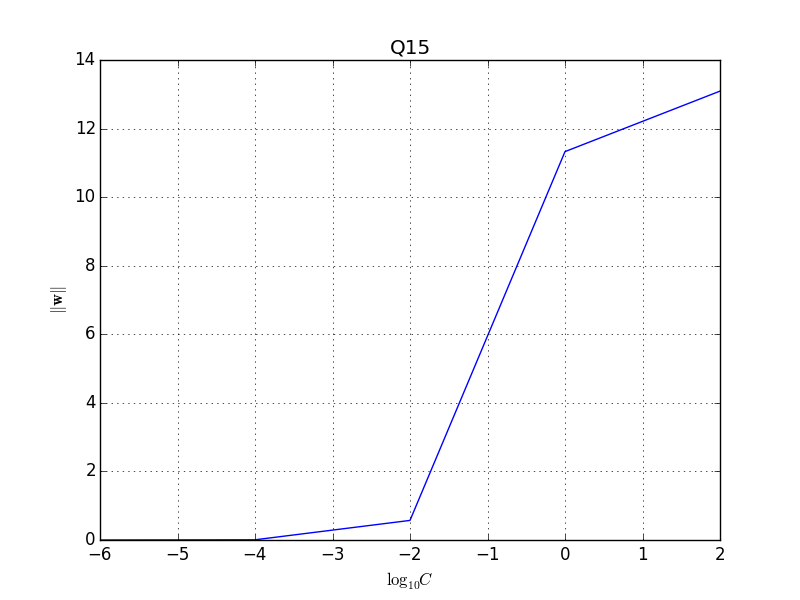
\includegraphics[scale=0.5]{Q15.png}
	\caption{Q15}
	\label{Q15}
\end{figure}
As $C$ becomes larger, $\VecAbsVal{\BF{w}}$ becomes larger, too.

\QEDB

\horrule{0.5pt}

\subsection*{Problem 16}

All $E_{\text{in}}$ versus $\log_{10}\ParTh{C}$ is $\SciNum{7.434}{-2}$.
\begin{figure}[H]
	\centering
	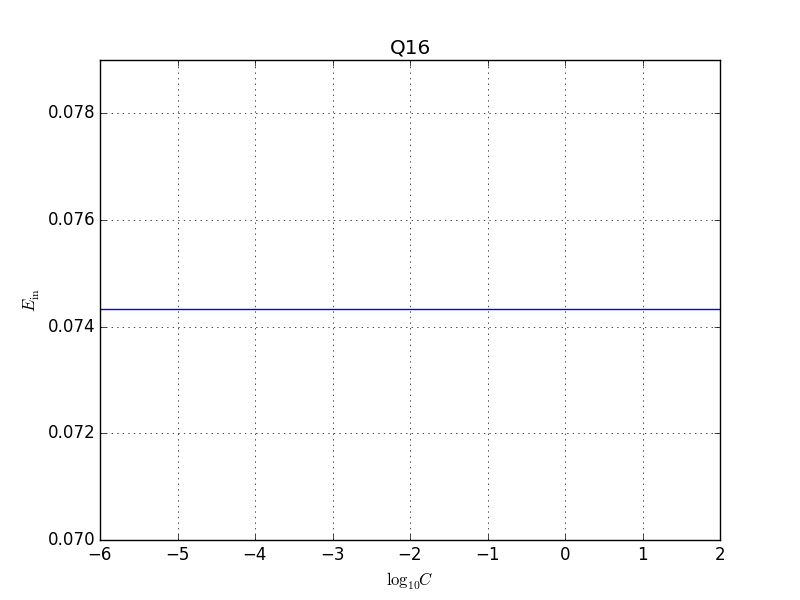
\includegraphics[scale=0.5]{Q16.png}
	\caption{Q16}
	\label{Q16}
\end{figure}
$E_{\text{in}}$ is independent of $C$.

\QEDB

\horrule{0.5pt}

\subsection*{Problem 17}

%All $\sum_{n=1}^{N}\alpha_n$ versus $\log_{10}\ParTh{C}$ is $\SciNum{1.084}{1}$.
\begin{align}
\sum_{n=1}^{N}\alpha_n\text{ list}=\SBrackets{\SciNum{1.084}{-3}, \SciNum{1.084}{-1}, \SciNum{1.084}{1}, \SciNum{1.084}{3}, \SciNum{1.084}{5}}
\end{align}
\begin{figure}[H]
	\centering
	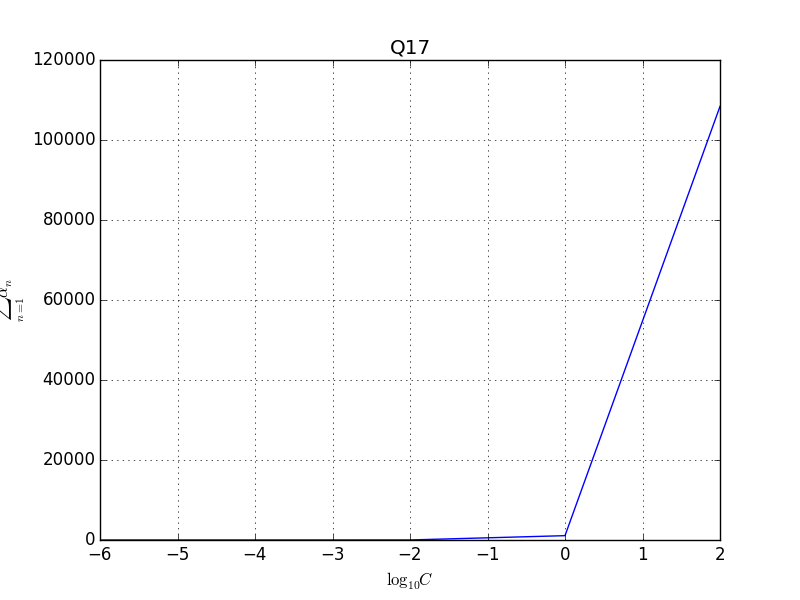
\includegraphics[scale=0.5]{Q17.png}
	\caption{Q17}
	\label{Q17}
\end{figure}
From this figure, we have
\begin{align}
\sum_{n=1}^{N}\alpha_n\propto C
\end{align}

\QEDB

\horrule{0.5pt}

\subsection*{Problem 18}

\begin{align}
\text{margin list}=\SBrackets{3.607, \SciNum{3.577}{-1}, \SciNum{5.182}{-2}, \SciNum{3.210}{-2}, \SciNum{3.068}{-2}}
\end{align}
\begin{figure}[H]
	\centering
	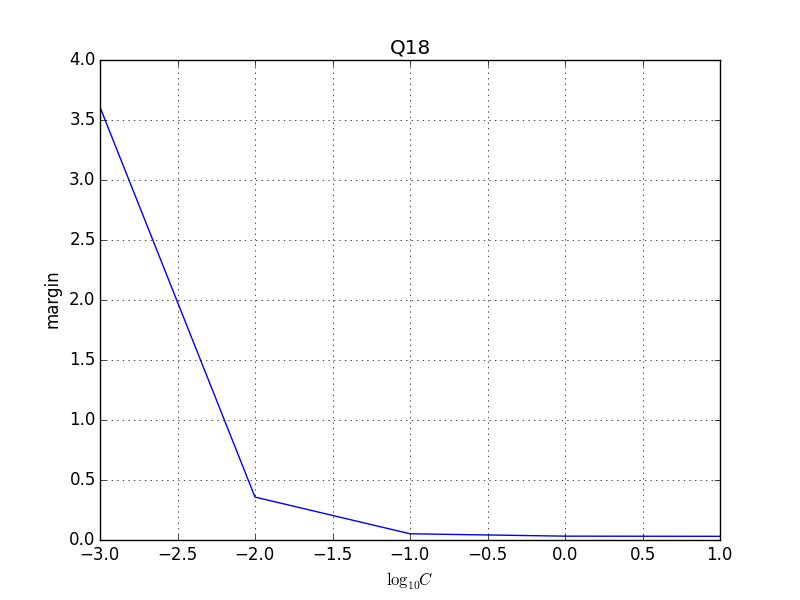
\includegraphics[scale=0.5]{Q18.png}
	\caption{Q18}
	\label{Q18}
\end{figure}
The margin is strictly decreasing as $C$ becomes larger.

\QEDB

\horrule{0.5pt}

\subsection*{Problem 19}

\begin{align}
E_{\text{out}}\text{ list}=\SBrackets{\SciNum{1.071}{-1}, \SciNum{9.915}{-2}, \SciNum{1.051}{-1}, \SciNum{1.789}{-1}, \SciNum{1.789}{-1}}
\end{align}
\begin{figure}[H]
	\centering
	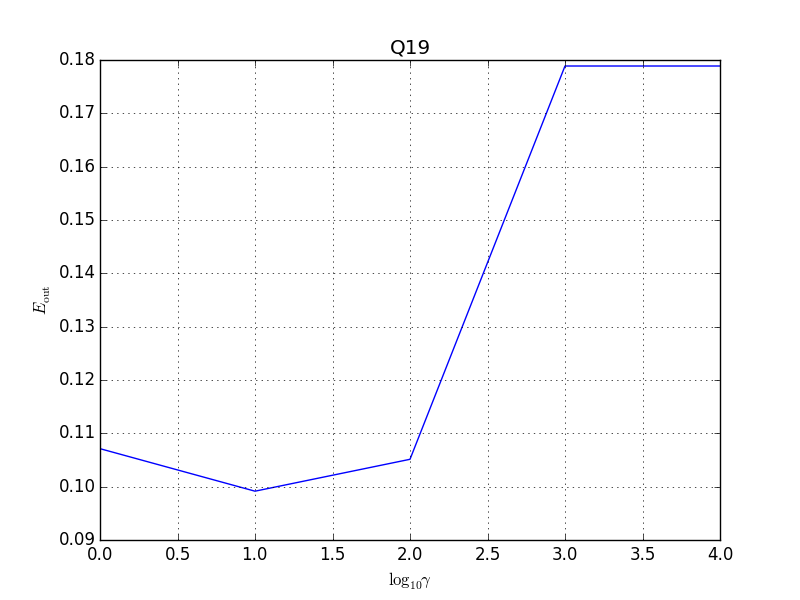
\includegraphics[scale=0.5]{Q19.png}
	\caption{Q19}
	\label{Q19}
\end{figure}
The minimum occurs at $\gamma=10$. $E_{\text{out}}$ becomes larger as $\gamma$ becomes larger.

\QEDB

\horrule{0.5pt}

\subsection*{Problem 20}

The corresponding $\gamma$ of $\min E_{\text{val}}$ are 10 in 99 results, one result is 1.
\begin{figure}[H]
	\centering
	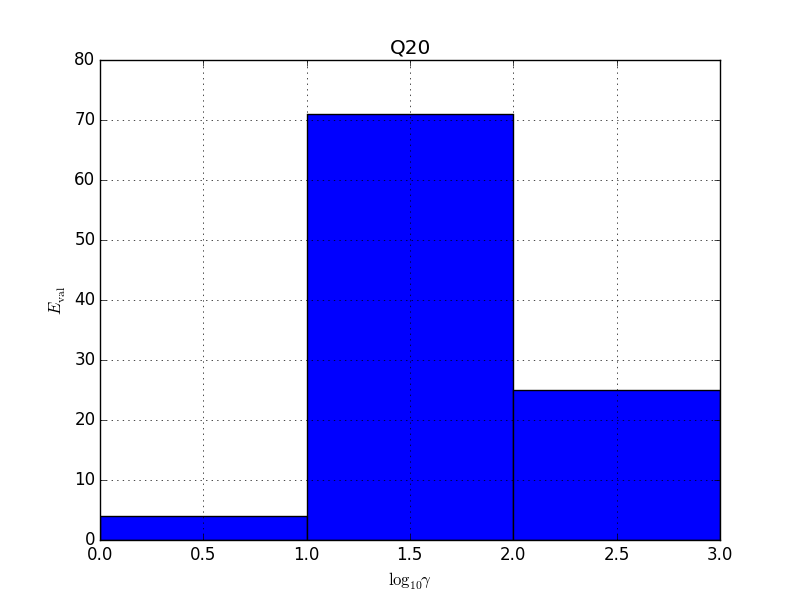
\includegraphics[scale=0.5]{Q20.png}
	\caption{Q20}
	\label{Q20}
\end{figure}
Over almost all random choices, $\gamma=10$ always minimizes $E_{\text{val}}$.

\QEDB

\horrule{0.5pt}

\section*{Reference}

\begin{enumerate}

\item[{[1]}] Lecture Notes by Hsuan-Tien LIN, Department of Computer Science and Information Engineering, National Taiwan University, Taipei 106, Taiwan.

\item[{[2]}] Quadratic Programming with Python and CVXOPT

\url{https://courses.csail.mit.edu/6.867/wiki/images/a/a7/Qp-cvxopt.pdf}

\end{enumerate}

\end{document}